\chapter{Abstractions}
While Spark.ML and other machine learning libraries provide abstractions for various machine
learning concepts like cost functions and optimizers, they do not have any abstractions
that are suitable for representing the model building process.

Therefore, ModelDB S+C must develop its own set of abstractions that can represent
the different operations for model building. These abstractions must be simple so
that they are easily understood and not too difficult to implement. Since ModelDB
Server aims to be library agnostic, they must be general enough to be applied to
a number of different machine learning libraries. Finally, since it is impossible,
to anticipate all the model building operations that a user may be interested in,
the abstractions must be composable and flexible so that new abstractions can be built 
from them that can represent other pieces of the model building process.

This chapter describes the abstractions in ModelDB S+C, building up from the
simplest abstractions to the higher level ones.

ModelDB S+C stores data in a SQL database (currently, a SQLite database is
used). Each abstraction below will be listed with its corresponding SQL 
tables, if any exist. 

The SQL tables below have been simplified in order to focus on the pieces 
of the table that are important for understanding the abstractions. Consequently,
some details like indices, non-nullity constraints, primary key columns, 
non-essential columns, and more have been omitted.


\section{Primitives}
ModelDB S+C is built on three primitives: the DataFrame, Transformer, and 
TransformerSpec.

\subsection{DataFrame}

A DataFrame represents a table of data. It has a number of named, typed columns
and it stores a count of rows. It is represented using the tables below.

\begin{minted}{sql}
CREATE TABLE DataFrame (
  numRows INTEGER,
  dataSource TEXT
);

CREATE TABLE DataFrameColumn (
  dfId INTEGER REFERENCES DataFrame,
  name TEXT,
  type TEXT,
  columnIndex INTEGER
);
\end{minted}

Again, recall that a number of details (e.g. primary key column) have been omitted
for brevity. The DataFrame table stores the number of rows, which is useful for
understanding the sizes of various DataFrames used in the model building process.
It also indicates its data sources, which could be a CSV in the local filesystem,
a JSON file stored on HDFS, or something else altogether. Since users may store
data in a variety of formats and locations, a DataFrame cannot make any assumptions
about what the data looks like or where it lives. The columns of a DataFrame
are stored in another table called DataFrameColumn. Each DataFrame column simply
points to its associated DataFrame and provides the name, type, and numerical index
(e.g. 0 for first column, 1 for second column) of the column. Observe that ModelDB S+C does
not place any restrictions on the allowed types in a DataFrame, because this
can vary across machine learning libraries. One notable aspect of ModelDB S+C
is that it only stores metadata about a DataFrame, rather than the actual rows.
The reasoning here is that a user's dataset could be very large, and importing it
into ModelDB S+C would be intractable. Additionally, storing the data in ModelDB
S+C would limit the user's freedom to store data in the locations and file formats
that best suit their application. However, by storing the dataSource column for
each DataFrame, the user is given a pointer to the underlying data, which they can
load with the tool of their choice.

\subsection{Transformer} 
The DataFrame abstraction describes the data involved in the model building process.
The Transformer abstraction, on the other hand, describes the operations that can
be performed on that data. A Transformer is an object that can takes an input DataFrame
and produces an output DataFrame. Its tables are shown below:

\begin{minted}{sql}
CREATE TABLE Transformer (
  transformerType TEXT,
  filepath TEXT
);

CREATE TABLE Feature (
  name TEXT,
  featureIndex INTEGER,
  importance DOUBLE,
  transformer INTEGER REFERENCES TRANSFORMER
);
\end{minted}

The Transformer table is quite simple, just storing a type (e.g. OneHotEncoder,
LinearRegressionModel) and a path to the file containing the serialized Transformer.
This is again done to maximize flexibility. ModelDB S+C does not impose any restrictions
on the kinds of Transformers that can be stored, as different machine learning libraries
may store different kinds of transformers. By storing the filepath to the serialized Transformer,
the user is able to load the Transformer into their machine learning library of choice and use
it to make predictions. Many machine learning libraries, including Spark.ML and Scikit-learn offer
facilities for serializing and deserializing Transformers. Transformers include features, which are the
columns they expect as inputs. Each feature has a name, index (in the feature vector), and importance. 
Notice that a Transformer does not have to be a machine learning model, like a logistic regression model. 
It can also be a data pre-processor, like
a one-hot encoder. One reasonable criticism of the Transformer table is that its simplicity 
prevents the user from storing useful model parameters, like the weights of a linear regression model,
that they may want to query. This is not an issue, however, because it is possible to create
additional tables on top of Transformer which support this information (as in the case of LinearModel
and TreeModel, which will be described later in this chapter).

\subsection{TransformerSpec}
The final primitive in ModelDB S+C is the TransformerSpec. Some Transformers, which
ModelDB S+C calls models are created by fitting a DataFrame where the fitting is 
guided by a set of hyperparameters. These hyperparameters are stored in a 
TransformerSpec, whose tables are shown below.

\begin{minted}{sql}
CREATE TABLE TransformerSpec (
  transformerType TEXT
);

CREATE TABLE HyperParameter (
  spec INTEGER REFERENCES TransformerSpec,
  paramName TEXT,
  paramType TEXT,
  paramValue TEXT,
  paramMinValue REAL,
  paramMaxValue REAL
);
\end{minted}

The TransformerSpec table is very simple, it just indicates the kind of Transformer
being specified. Each HyperParameter points to its associated TransformerSpec and indicates
the name, type, value, and bounds for the hyperparameter. The bounds may be ignored
for non-numerical hyperparameters. Notice that this allows expressing a wide range
of hyperparameters such as the regularization parameter of a linear regression model, 
the number of trees in a random forest, or the optimization algorithm (e.g. stochastic 
gradient descent) used to train a logistic regression model.

It is worth noting that the Transformer table does not reference the TransformerSpec
table and that the TransformerSpec table does not reference the Transformer table. This
is for two reasons. First, some Transformers can be created without specifying any
hyperparameters (e.g. a Transformer that removes all rows containing null values). 
Second, a user may want to create a TransformerSpec that lives independently of any
Transformer. For example, suppose that a user has defined a set of hyperparameters to
train a random forest model, and that they receive new datasets every week. They may choose
to re-use the same TransformerSpec for each week of data. Consequently, the TransformerSpec is
not tied to just one Transformer and can even be tied to zero Transformers when it is first created. With
all this being said, there does exist a mechanism by which ModelDB S+C indicates that a Transformer
was produced from a given TransformerSpec, and that is the FitEvent, which is introduced later in
this chapter.

DataFrame, Transformer, and TransformerSpec are very simple abstractions, but are powerful in that
they can express a huge variety of datasets, models/data preprocessors, and model training configurations.
Equally important is the fact that they are also present, in some capacity, in many other machine learning
libraries.

\section{Syncable Events}
ModelDB S+C is designed with the assumption that most of the interesting operations in
model building can be represented as combinations of the three primitives described in the
previous section. A specific operation that occurs in the user's model building process
is called a Syncable Event ("Syncable" because it is shared between server and client, 
"Event" because it is a specific operation performed at a specific time). The following
sections describe several of these Syncable Events. Each Syncable Event receives its own
table (or few tables) in the database and Syncable Events can be composed together to
create other events. All of the Syncable Events that have that ModelDB S+C has stored
are referenced in the Event table, which is shown below.

\begin{minted}{sql}
CREATE TABLE Event (
  eventType TEXT,
  eventId INTEGER
);
\end{minted}

An Event includes a type (e.g. "fit", "transform") and the ID of the event
in its corresponding table.

\section{Core Events}
The three foundational Syncable Events are TransformEvent, FitEvent, and MetricEvent.

\subsection{TransformEvent}
A TransformEvent represents the creation of a new DataFrame from an old DataFrame by
applying a Transformer. This is a very general idea and can be used to represent both
data pre-processing steps and prediction-making with a model.

The TransformEvent table has the following schema:

\begin{minted}{sql}
CREATE TABLE TransformEvent (
  oldDf INTEGER REFERENCES DataFrame,
  newDf INTEGER REFERENCES DataFrame,
  transformer INTEGER REFERENCES Transformer,
  inputColumns TEXT, -- Should be comma-separated, no spaces, alphabetical.
  outputColumns TEXT -- Should be comma-separated, no spaces, alphabetical.
);
\end{minted}

The event indicates both the old and new DataFrames, the Transformer performing
the transformation, and the input and output columns. The input and output columns
could also be represented in their own tables, rather than as strings. This may
be worth doing in the future because it would more easily enable queries such as
finding the TransformEvent that produced a given column in a DataFrame.

To understand the flexibility of TransformEvent, it is worth considering a few
sample operations that it can represent. First, consider one-hot encoding. One-hot
encoding is a technique for converting categorical variables into binary vectors.
If a categorical variable with $k$ levels, then level $l$ can be indicated with
a vector with $k$ entries where the $l^{th}$ entry is 1 and the other entries are
0. To represent one-hot encoding of a column, "col", we can create a Transformer of
type OneHotEncoder. Then, we can create a TransformEvent where the input column
is marked as "col" and the output column is marked as "oneHotEncodedCol". Notice,
that the old and new DataFrames in the TransformEvent only need to be logically, rather
than physically, distinct. Therefore, the underlying machine learning library may
actually use the same chunk of memory to represent data that is common to the two 
DataFrames. Consider another example - making a prediction with a model. In this
case, the model can be the Transformer, the input columns are the feature names,
and the output column can contain the prediction (and perhaps there can be another
column that contains a confidence level in that prediction). As a final example,
consider a transformation that removes rows from a DataFrame that contain null values.
The "null remover" can be a Transformer, the input and output columns can be empty
strings, and the old and new DataFrames can have identical columns, but a differing
number of rows. Thus, TransformEvent is a very flexible abstraction that can represent
a wide range of operations.

\subsection{FitEvent}

The second core Syncable Event is the FitEvent, which represents the fitting of a
DataFrame with a TransformerSpec to produce a Transformer.

\begin{minted}{sql}
CREATE TABLE FitEvent (
  transformerSpec INTEGER REFERENCES TransformerSpec,
  transformer INTEGER REFERENCES Transformer,
  df INTEGER REFERENCES DataFrame,
  predictionColumns TEXT, -- Should be comma-separated, no spaces, alphabetical.
  labelColumns TEXT, -- Should be comma-separated, no spaces, alphabetical.
  problemType TEXT 
);
\end{minted}

The FitEvent is the main abstraction that represents the building of a model. It
indicates the data used to produce the model, the specification that guided training,
and the produced model. It indicates the label columns that were used to teach the
model, the columns in which the model will output its prediction, and the type of
problem (e.g. regression, binary classification) that the model solves. Indeed, it
is possible at this point to clearly define what a model is in ModelDB S+C. A model is
a Transformer with an associated FitEvent. 
Notice that the feature columns are not included because they are already stored in the Feature
table. 

\subsection{MetricEvent}
Thus far, the chapter has explained how ModelDB S+C represents the operations that create data (TransformEvent)
and operations that create models (FitEvent). Another potential output of an operation is a statistic, metric, or
other number that describes or evaluates a dataset or model. For this purpose, ModelDB S+C includes a Syncable Event
called MetricEvent.

\begin{minted}{sql}
CREATE TABLE MetricEvent (
  transformer INTEGER REFERENCES Transformer,
  df INTEGER REFERENCES DataFrame,
  metricType TEXT,
  metricValue REAL
);
\end{minted}

The above representation is quite flexible, in that it allows metrics on datasets as well as
metrics on models. For example, consider the problem of finding a the standard deviation of a column.
This could be represented by a MetricEvent where metricType is "standard deviation", the metricValue
is the actual numeric value for the standard deviation, the transformer is a StandardDeviationComputer (with
one feature column - the column for which the standard deviation is being computed), and the df is the
DataFrame with the column for which the standard deviation is being computed. As another example, consider
the problem of evaluating a model's prediction accuracy. In this case, the transformer could be the model being
evaluated, the df could be the DataFrame for which the model made predictions, the metricType could be "accuracy",
and the metricValue could be the actual accuracy score.

TransformEvent, FitEvent, and MetricEvent are the fundamental Syncable Events in ModelDB S+C. They build on the
ModelDB S+C's three primitives: DataFrame, Transformer, and TransformerSpec. While these Syncable Events are powerful on
their own, they can also be combined together to represent higher level events.

\section{Composite Events}
ModelDB S+C includes a number of other events which combine the three core Syncable Events and the three primitives.
For brevity, only the most interesting events will be discussed in this paper.

\subsection{CrossValidationEvent}
Cross validation is a model selection operation that is an integral part of the
model building process. Recall that cross validation involves considering a hyperparameter
configuration, breaking a DataFrame into pieces (folds), training a model for each fold (it
is trained on all folds except one), and evaluating a model for each fold (it is evaluated on
the fold that was left out for training). This operation is represented using the following tables:

\begin{minted}{sql}
CREATE TABLE CrossValidationEvent (
  df INTEGER REFERENCES DataFrame,
  spec INTEGER REFERENCES TransformerSpec
);

CREATE TABLE CrossValidationFold (
  metric INTEGER REFERENCES MetricEvent NOT NULL,
  event INTEGER REFERENCES CrossValidationEvent NOT NULL,
);
\end{minted}

The two simple tables above are all that is needed to allow ModelDB S+C to store
cross validation events. They are deceptively simple because ModelDB S+C leverages
the three primitives and three core Syncable Events heavily when representing cross validation.
To illustrate, consider the diagrammatic representation of cross validation in Figure
\ref{fig:cross_validation_event} (only one fold has been shown to avoid making the diagram too large).

\begin{figure}
  \centering
  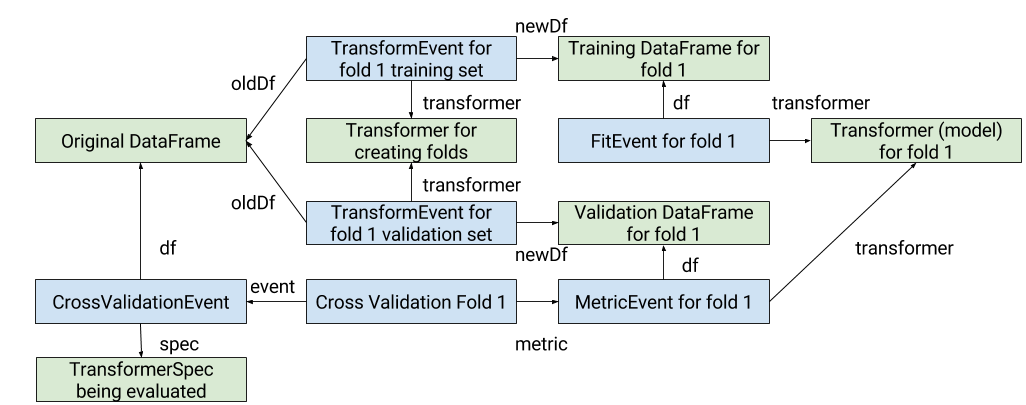
\includegraphics[width=7.0in]{cross_validation_event}
  \caption{
    Diagrammatic representation of cross validation in ModelDB S+C. Green boxes
    represent primitives and blue boxes represent Syncable Events. Arrows
    represent foreign key relationships.
  }
  \label{fig:cross_validation_event}
\end{figure}

To understand Figure \ref{fig:cross_validation_event}, it is best to start at the CrossValidationEvent.
The CrossValidationEvent points to the TransformerSpec (i.e. hyperparameter configuration) that is being evaluated
as well as to the full DataFrame that is being evaluated. There is one CrossValidationFold that points to the
CrossValidationEvent. The fold points to the MetricEvent that contains its evaluation metric. The MetricEvent
points to the model (Transformer) that was trained when the fold was excluded and to the validation DataFrame
on which the metric was computed. The validation DataFrame was produced from the original DataFrame using a special
Transformer that creates folds. The model for the fold was created via a FitEvent that points to the training DataFrame
for the fold. The training DataFrame for the fold was created from the original DataFrame using the same special Transformer that
creates folds.

Thus, the complex process of cross validation can be represented with ModelDB S+C by adding two simple tables and cleverly
combining the primitives and core Syncable Events.

\subsection{GridSearchCrossValidationEvent}
The cross validation operation is often combined with a grid search, in which several hyperparameter configurations
are evaluated and cross validation is performed for each one. Then, the best hyperparameter configuration (i.e. the one with the largest
average evaluation metric) is selected and used to train a model on the entire dataset. This is a complex process, but can be easily
supported in ModelDB S+C by adding the following two tables.

\begin{minted}{sql}
CREATE TABLE GridSearchCrossValidationEvent (
  best INTEGER REFERENCES FitEvent,
);

CREATE TABLE GridCellCrossValidation (
  gridSearch INTEGER REFERENCES GridSearchCrossValidationEvent,
  crossValidation INTEGER REFERENCES CrossValidationEvent
);
\end{minted}

The GridSearchCrossValidationEvent table simply stores a reference to a FitEvent
that produced the final model (a Transformer) by using the best TransformerSpec to
train on the entire original DataFrame. Then, GridCellCrossValidations are created
(one for each hyperparameter configuration that was considered) and each points to
the CrossValidationEvent for its corresponding hyperparameter configuration.

Looking back, the prefix "GridSearch" is actually a misnomer, because there is nothing about the
above abstraction that requires a grid search to be performed. The abstraction above
can represent grid search, random search, and various other model selection strategies that
consider a number of hyperparameter configurations.

\subsection{PipelineEvent}
One common practice in Spark.ML, Python Scikit-learn, and perhaps other machine learning
libraries is that of building a preprocessing pipeline. For example, consider the simple
preprocessing pipeline in Figure \ref{fig:preprocessing_pipeline}. This pipeline assumes
that the machine learning library includes Transformer objects that produce an output DataFrame
from an input DataFrame and Estimator objects that apply a TransformerSpec on a DataFrame to create
a Transformer. Spark.ML and Python Scikit-learn both include Transformers and Estimators. The user
arranges Estimators and Transformers into a chain, called a Pipeline, feeds in a DataFrame, and the result is a chain
of Transformers. This chain of Transformers, or Pipeline Model, can be used in other parts of the 
program. Notice that if the final piece of the Pipeline an Estimator that produces a model, then
the user may be able to represent their entire machine learning system using a Pipeline Model. They can also
add post-processing steps by adding more Transformers at the end.

\begin{figure}
  \centering
  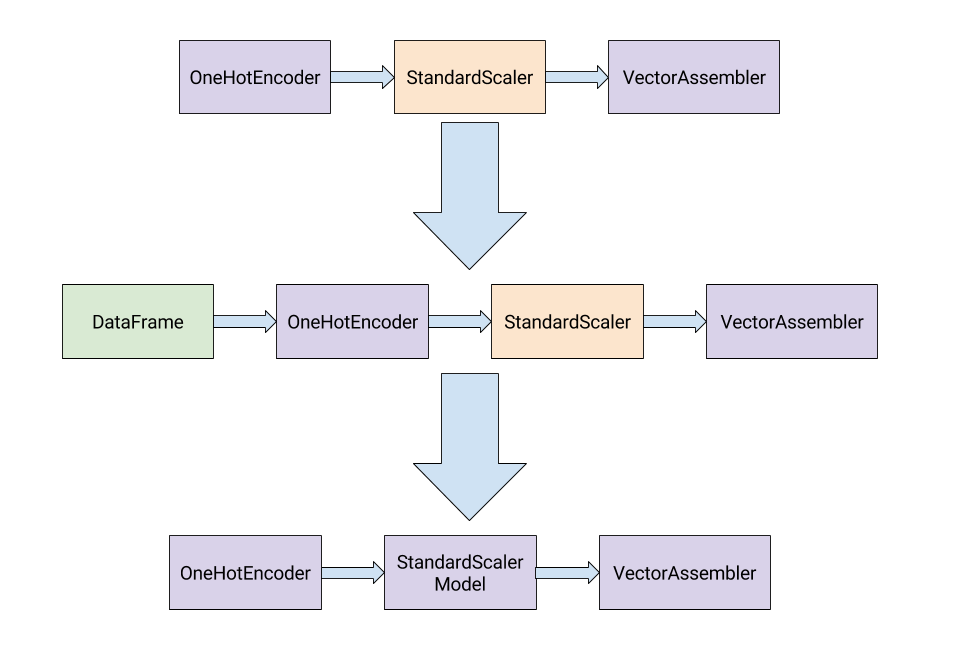
\includegraphics[height=3.0in]{preprocessing_pipeline}
  \caption{
    Creation of a pre-processing pipeline. First, the user chains together some
    Transformers and Estimators (objects that can apply their TransformerSpec to
    create a Transformer from a DataFrame). Next, the user feed a DataFrame into the pipeline. The
    Transformers transform their input DataFrame, produce an output DataFrame, and
    pass the output on to the next step in the pipeline. The Estimators use the input DataFrame
    to create a Transformer, and then they replace themselves with this Transformer - the
    Transformer then transforms the input DataFrame and passes the output to the next step.
  }
  \label{fig:preprocessing_pipeline}
\end{figure}

ModelDB S+C represents the creation of Pipelines using the following table:

\begin{minted}{sql}
CREATE TABLE PipelineStage (
  pipelineFitEvent INTEGER REFERENCES FitEvent,
  transformOrFitEvent INTEGER REFERENCES Event,
  isFit INTEGER, -- 0 if transform stage and 1 if this is a fit stage.
  stageNumber INTEGER 
);
\end{minted}

First, ModelDB S+C represents the creation of a Pipeline Model (which is a Transformer) from
a DataFrame using a FitEvent. The TransformerSpec associated with this FitEvent can have an empty
set of HyperParameters. Then, the pipeline creation is broken into "stages". A stage is either a 
"transform stage" or a "fit stage". A transform stage is a TransformEvent where a Transformer in the pipeline
transforms its input and forwards the output to the next step. A fit stage is when an Estimator creates a Transformer
by applying its TransformerSpec to its input DataFrame. Notice that each Estimator in the user's pipeline produces
one fit stage and one transform stage. The stages are ordered using the stageNumber, which should be higher for later
stages.

The transformOrFitEvent and isFit fields are used to distinguish the stage as a transform stage or fit stage. Admittedly,
this is a bit inelegant. A cleaner solution would be the following:

\begin{minted}{sql}
CREATE TABLE PipelineStage (
  pipelineFitEvent INTEGER REFERENCES FitEvent,
  transformStage INTEGER REFERENCES TransformEvent,
  fitStage INTEGER REFERENCES FitEvent,
  stageNumber INTEGER 
);
\end{minted}

In this case, every Estimator and every Transformer in the Pipeline would produce a PipelineStage. For the Estimators,
the fitStage would point to their creation of a Transformer by applying their TransformerSpec on their input DataFrame.
For the Estimators, the transformStage would point to the transformation of their input DataFrame into an output DataFrame 
using the Transformer that was created. For a Transformer, the transformStage would be its application to the input DataFrame
to produce an output DataFrame and its fitStage would be NULL.

\subsection{Annotation}
The above events demonstrate how ModelDB S+C is able to express complex model building operations by
cleverly combining its primitives and core events. There are more such events (e.g. RandomSplitEvent) in
ModelDB S+C which are similar in nature, but which will not be discussed here for brevity.

Another composite event of interest, however, is the Annotation, which does not simply represent
an existing model building operation, but actually enables new functionality. ModelDB Spark Client allows the user
to make notes for themselves and link these notes to DataFrames, Transformers, and TransformerSpecs. This can be done
with Scala code like the following:

\begin{minted}{scala}
  ModelDbSyncer.get.annotate(
    "I'm getting poor performance on", 
    testDf1, 
    "with model", 
    model1, 
    "Is there a bug with this model? Should investigate tomorrow."
  )
\end{minted}

The Scala code sample above stores an Annotation in ModelDB S+C, which involves
the following tables:

\begin{minted}{sql}
CREATE TABLE Annotation (
  posted TIMESTAMP
);

CREATE TABLE AnnotationFragment (
  annotation INTEGER REFERENCES Annotation,
  fragmentIndex INTEGER,
  transformer INTEGER REFERENCES Transformer,
  dataFrame INTEGER REFERENCES DataFrame,
  spec INTEGER REFERENCES TransformerSpec,
  message TEXT,
);
\end{minted}

An Annotation indicates the time it was created and is associated with a number
of AnnotationFragments. The AnnotationFragments are ordered using the fragmentIndex
column. A fragment can either contain text, a reference to a Transformer, a reference
to a DataFrame, or a reference to a TransformerSpec (in Spark.ML code, this would
correspond to an Estimator), The Scala code above would result in the creation
of five AnnotationFragments, where the first, third, and fifth store text, the second
refers to a DataFrame, and the fourth refers to a Transformer.

In hindsight, Annotation should be called AnnotationEvent in order to make
it consistent with the "Event" suffix associated with other Syncable Events.

\section{Linear and Tree Models}

While ModelDB S+C does allow the user to serialize their models to a filesystem,
the description of the abstractions so far does not allow querying of the models
because the Transformer table is so simple. To make querying possible, ModelDB S+C
includes additional tables that build off the Transformer table to support storage
(and querying) of additional model data. Specifically, ModelDB S+C has tables for
linear models and tree models, which are designed to support the logistic regression,
linear regression, decision tree, gradient boosted tree, and random forest models in
Spark.ML.

\subsection{Linear Models}

Linear models are defined by their vector of weights. These weight vectors are
stored with the following table.

\begin{minted}{sql}
CREATE TABLE LinearModelTerm (
    model INTEGER REFERENCES Transformer,
    termIndex INTEGER,
    coefficient DOUBLE,
    tStat DOUBLE,
    stdErr DOUBLE,
    pValue DOUBLE
);
\end{minted}

A linear model is represented by a Transformer, and its weights are represented
by the associated LinearModelTerms. Each term indicates the weight (the coefficient) and
some statistics about the weight (t-statistic, standard error, and p-value). The position
of the weight in the weight vector is given by termIndex (which is 0 if there is an intercept
term).

This table makes it possible to run some useful queries (e.g. build confidence intervals
aroudn the weights) and also makes it possible to develop tools to reconstruct linear models
based on the weights and the transformerType.

The actual implementation of ModelDB S+C includes a table called LinearModel, but this
is there for legacy purposes and is not actually needed (its rmse, r2, and explainedVariance 
columns can be stored in MetricEvents rather than as columns).

\subsection{Tree Models}
A decision tree consists of nodes and edges (or links) between them. ModelDB S+C represents
this using the following tables:

\begin{minted}{sql}
CREATE TABLE TreeNode (
  isLeaf INTEGER, -- 1 if node is leaf, 0 if node is internal
  prediction DOUBLE, -- Internal nodes obviously do not use their predictions
  impurity DOUBLE, -- Impurity of node.
  gain DOUBLE, -- Information gain at node. NULL for leaf nodes.
  splitIndex INTEGER, -- Index of feature that the internal node is splitting. 
                      -- NULL if this is a leaf node.
  rootNode INTEGER REFERENCES TreeNode -- NULL for the root node
);

DROP TABLE IF EXISTS TreeLink;
CREATE TABLE TreeLink (
  parent INTEGER REFERENCES TreeNode,
  child INTEGER REFERENCES TreeNode,
  isLeft INTEGER NOT NULL -- 1 if the child is a left child 
                          -- 0 if the child is a right child.
);
\end{minted}

Nodes indicate whether they are leaves. Leaf nodes indicate their prediction, 
impurity, and the root node of the tree (unless they are the root). 
Internal nodes indicate their gain, impurity, the feature they are splitting, 
and their root (unless they are the root). This table could be augmented so
that internal nodes also store the splitting criterion (i.e. how to decide which
child to forward an input example to), but this is not utilized in ModelDB S+C so
it is currently omitted. 

The TreeLink table simply indicates a parent child relationship. Spark.ML's 
decision trees are binary trees, and ModelDB S+C uses the same. However, for 
generalization to non-binary trees, the isLeft column could be replaced by a childIndex
column that indicates the index (0 being leftmost) of the child.

Random forests and gradient boosted trees are ensembles of decision trees, where
each tree is given some weight. In fact, a decision tree can be thought of as an
ensemble consisting of a single tree that gets all the weight. With this in mind, ModelDB S+C
defines the following tables:

\begin{minted}{sql}
CREATE TABLE TreeModel (
  model INTEGER REFERENCES Transformer,
  modelType TEXT NOT NULL -- Should be "Decision Tree", "GBT", or "Random Forest"
);

CREATE TABLE TreeModelComponent (
  model INTEGER REFERENCES Transformer,
  componentIndex INTEGER,
  componentWeight DOUBLE,
  rootNode INTEGER REFERENCES TreeNode
);
\end{minted}

A TreeModel simply indicates the associated Transformer and the type of the model.
The model is associated with a number of trees through the TreeModelComponent, which
indicates the tree's numerical order in the overall ensemble (componentIndex), the
tree's weight, and the root node of the tree. A decision tree can be thought of as
TreeModel with a single TreeModelComponent.

While the above tables are designed for tree ensembles specifically, they could be
extended to support ensemble models in general.

\section{ModelDB Syncer}
ModelDB Syncer is a client side abstraction for recording events and sending them
to ModelDB Server. When operations (e.g. creation of a model, splitting of a DataFrame)
are detected by the ModelDB Spark Client, a SyncableEvent object is created and sent to
a global ModelDB Syncer object. This ModelDB Syncer maintains an ordered buffer of Syncable Events
that it periodically flushes to the ModelDB Server. Each Syncable Event is imbued with logic for converting
the Spark objects it represents into the corresponding ModelDB S+C abstraction and sending that information to
ModelDB Server. The ModelDB Syncer performs other roles as well, such as maintaining a mapping between Spark
objects and their IDs in ModelDB S+C. The ModelDB Syncer will be described in greater detail in the Implementation chapter.
